\documentclass{article}


\usepackage{arxiv}

\usepackage[utf8]{inputenc} % allow utf-8 input
\usepackage[T1]{fontenc}    % use 8-bit T1 fonts
\usepackage{hyperref}       % hyperlinks
\usepackage{url}            % simple URL typesetting
\usepackage{booktabs}       % professional-quality tables
\usepackage{amsfonts}       % blackboard math symbols
\usepackage{nicefrac}       % compact symbols for 1/2, etc.
\usepackage{microtype}      % microtypography
\usepackage{lipsum}
\usepackage{graphicx}
\usepackage{todonotes}

\title{The Sankoff Algorithm for Phylogeographics}


\author{
  Julia Fischer \\
  Universität Tübingen \\
  \texttt{juli.fischer@student.uni-tuebingen.de} \\
  6039174 \\
  \And
  Peter Heringer \\
  Universität Tübingen \\
  \texttt{peter.heringer@student.uni-tuebingen.de} \\
  6109174 \\
  \And 
  Michael Mederer \\
  Universität Tübingen \\
  \texttt{michael.mederer@student.uni-tuebingen.de} \\
  XXXXXXX \\
  \And 
  Felix Seidel \\
  Universität Tübingen \\
  \texttt{felix.seidel@student.uni-tuebingen.de} \\
  5969276 \\
}

\begin{document}
\maketitle

\begin{abstract}
\end{abstract}


\section{Introduction}
Given a rooted tree $T$ with labeled leaves, the small parsimony problem is about
finding labels for the internal nodes of the tree such that the changes from an
internal nodes to all of its children are minimal
\cite{jonesIntroductionBioinformaticsAlgorithms2004}.
Among others, the Sankoff algorithm can be used to solve the small parsimony
problem \cite{sankoffMinimalMutationTrees1975}. 

Sankoff's algorithm is designed to use an already existing phylogenetic tree with labeled leaves and
some form of cost matrix to label the internal nodes in a way that minimizes the cost based on the
matrix and underlying topology. For this the algorithm uses two phases: a
forward pass and a backward pass.
Starting with the parents of the leaves, the forward pass fills a
list detailing what choosing a certain label would incur in
cost for every node. For this, the cost for the transition from each possible state of the
parent to each possible state of the children must be calculated, which has an
estimated complexity of $\mathcal{O}(k^2)$ where $k$ is the number of possible
states. This calculation has to be done for each node in the tree, thus we
estimate the runtime of the forward pass
with $\mathcal{O}(nk^2)$ where $n$ is the number of nodes in the tree and $k$ is
the number of possible states each node can take.
The second part is the backward pass. Starting with the root, the algorithm
choses the correct label based on the cost lists. This results in the labeled
tree. For this, each node has to be visited once. Hence, we estimate the
complexity of the backward pass with $\mathcal{O}(nk)$ where $n$ is the number of
nodes in the tree and $k$ is the number of states each node can take.

The Sankoff algorithm is usually applied to the broader scope of
inferring phylogenetic trees using cost matrices that model the transition
between different DNA or RNA nucleotides
\cite{jonesIntroductionBioinformaticsAlgorithms2004}, i.e. solving the large parsimony problem. By
using different cost
matrices, the algorithm can also be used to model other biological questions,
for example in the Camin-Sokal-Parsimony \cite{caminMethodDeducingBranching1965}
or in the Dollo-Parsimony \cite{farrisPhylogeneticAnalysisDollo2022}. More
recently, the Sankoff algorithm was also used to infer the geographic origins of
the 2009 H1N1 pandemic using a distance matrix that represents the distances of
various international airports
\cite{reimeringPhylogeographicReconstructionUsing2020}. In this, the authors use
a phylogenetic tree that represents the relationship between different strains
of the virus and map each taxon to the airport that is closest to the sampling
location. Then, three different cost matrices are utilized:

\begin{enumerate}
  \item Equal distance: Airports have a distance of 1 to each other
  \item Geographic distance: The actual geographic distances between different
  airports is used.
  \item Effective distances: An infection is more likely to spread from
  airport $A$ to airport $B$ if there are many people traveling from $A$ to
  $B$. Thus, the effective distances are calculated by using passenger data
  for each combination of airports.
\end{enumerate}

Using those cost matrices for airports and for the corresponding countries, the
labels for the internal nodes of the tree are calculated and, thus, their
geographic position.

One of the advantages in using the Sankoff algorithm for this problem as opposed to more
conventional approaches is, as the authors describe, a gain in performance. This is due to the fact
that the Sankoff algorithm is comparatively simple. Additionally, large parts can be implemented as
operations on matrices which can be done very quick in modern computers because of easy
parallelization and efficient libraries, such as BLAS \cite{lawsonBasicLinearAlgebra1979}. As
datasets can be quite large due to a large
amount of sequences and locations (in this case airports) having a fast
algorithm to even approximate the correct solution can be instrumental in getting a solution.

In the following report, we implement the method outlined in
\cite{reimeringPhylogeographicReconstructionUsing2020} and recreate the findings
by using the original data.

\section{Material and Methods}
The Sankoff algorithm was implemented using Python \todo{version number}
\cite{pythonsoftwarefoundationWelcomePythonOrg2023} and Numpy \cite{harrisArrayProgrammingNumPy2020}. Numpy was used to allow the use of
efficient matrix operations.

The base phylogenetic tree that we used is the H1N1 phylogeny described by
\cite{reimeringPhylogeographicReconstructionUsing2020}. For the calculations,
we've used the effective and geographic distance matrices from
\cite{reimeringDistanceMatricesParsimonious2019}. 

All visualizations (with the exception of visualizations from the original paper)\todo{Do we need
this?} were done using Python and Matplotlib \cite{MatplotlibVisualizationPython}. To accurately plot the maps and the locations of the
airports we used Geopandas \cite{GeoPandas12GeoPandas}. Additionally, we used the package airportsdata \cite{borsettiAirportsdataExtensiveDatabase2022} to get the locations of
airports and pycountry \cite{theunePycountryISOCountry} to translate letter codes
of countries.

To compare our implementation with the implementation that
was provided in \cite{reimeringPhylogeographicReconstructionUsing2020} in terms of runtime, we
executed the Sankoff implementation using the built-in command \texttt{time} on
a Linux notebook running \texttt{6.1.2-arch1-1} with a four core Intel(R) Core(TM) i5-
10210U CPU @ 1.60GHz CPU and 16G RAM for the geographic distance matrix for airports.

We calculated Fr\'{e}chet distances as a measure of comparing our results to the ones from \cite{reimeringPhylogeographicReconstructionUsing2020}. For the calculation we used the implementation provided by the authors \cite{reimeringFrechetTreeDistance2018}.

\section{Results}

\subsection{Labeled trees}
For the given input phylogeny, we've computed four different internal labelings: 
\begin{itemize}
    \item one based on the geographic distances between airports
    \item one based on the effective distances between airports
    \item one based on the geographic distances between countries
    \item one based on the effective distances between countries
\end{itemize}

Our tree that is based on the geographic distances between airports differs in
one node from the corresponding tree given in
\cite{reimeringPhylogeographicReconstructionUsing2020}, the trees that are based
on the effective geographic distances between airports are equal.

\subsection{Fr\'{e}chet distances}
\begin{itemize}
    \item Fr\'{e}chet tree distances used to quantify geographic differences between spread paths
    \item We compare our reconstructed trees with the ones from the paper
    \item by claculating discrete Fr\'{e}chet tree distances using geographic distances between locations
    \item method compares the paths of locations from the root of each leaf node, calculates discrete Fr\'{e}chet distances between them and corrects the distance for each node by the number of paths
\end{itemize}

Our inferred trees versus the trees from the paper:
\begin{itemize}
    \item geographic distances: 123.8497
    \item effective distances: 0
\end{itemize}

The Fr\'{e}chet distance between our trees:
\begin{itemize}
    \item effective airport vs geographic airport: 65149
    \item effective country vs geographic country: 12307.03
    \item airport to country comparison not possible due to distance matrix
\end{itemize}

\subsection{Runtime}
Our implementation of the Sankoff algorithm using the geographic distance
matrix for airports took \texttt{2m39.466s}, while the implementation provided in
\cite{reimeringPhylogeographicReconstructionUsing2020} took \texttt{6m32.557s}.
Our implementation is more than twice as fast for the $3865 \times 3865$
distance matrix than the original implementation.


\section{Discussion}
The Sankoff algorithm is rather easy to understand and can even be computed by
hand if the distance matrix and the tree are small. Also, for a given tree
topology, we've demonstrated that the computation of the labels of the internal
nodes is fast even for huge distance matrices such as the geographic and
effective distance matrices with $3865 \times 3865$ entries.

The tree that our implementation computed for the geographic airport matrices
differs in one label from the H1N1 tree given by
\cite{reimeringPhylogeographicReconstructionUsing2020}, i.e. we label the node
\texttt{intNode97} with \texttt{DTW} (Detroit Metro Airport) while they find the label
\texttt{IND} (Indianapolis International Airport).
This difference is the result of different prioritization in the implementation:
\texttt{intNode97} is the parent of three leaves, two of them labeled with
\texttt{DTW} and the third is labeled with \texttt{IND}. The parent of
\texttt{intNode97} is \texttt{intNode96} and has one additional child which is
also a leaf labeled with \texttt{IND}. The distance between \texttt{IND}
and \texttt{DTW} is $371.54$. Choosing either \texttt{IND} or \texttt{DTW} for
\texttt{intNode97} yields the same cost for choosing \texttt{IND} for
\texttt{intNode96}. Thus, from the perspective of maximum parsimony, both
choices are optimal. Moreover, the real-world implications of this concrete
difference should be small. Indianapolis and Detroit are cities that are close
to each other and as the sampling locations for the leaves are mapped to the
closest airport, there is already a certain amount of distortion
\todo{fuzziness? noise?} in the input data that has a comparable magnitude to
the difference between Indianapolis and Detroit.

Due to its fast computation, the Sankoff implementation enables rapid
experiments to plot the spread on the globe and to accelerate the discovery 
of the origin of a disease
(Figure~\ref{fig:world}). While the algorithmic inference of the origin must be
treated with caution, as it is not precise
\cite{reimeringPhylogeographicReconstructionUsing2020}, it is also worth noting
that in the case of global pandemics, the determination of the origin of the
disease can have undesired, societal implications if not treated with caution
\cite{chenPotentialImpactCOVID192020}.

If one is interested in how the disease was imported into a specific country or
region, the information that can be extracted from the labeling given by Sankoff
is limited: There might be many incoming routes to one airport or country. However,
the computed tree does not give any historical ordering, i.e. it does not
indicate which connection was first (Figure~\ref{fig:DEU0}).

\begin{figure}[!ht]
    \centering
    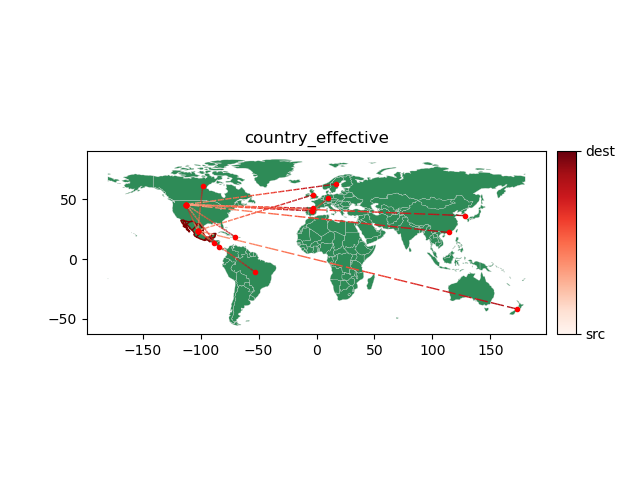
\includegraphics[width=0.8\linewidth]{world.png}
    \caption{World}%
    \label{fig:world}
\end{figure}

\begin{figure}[h!]
    \centering
    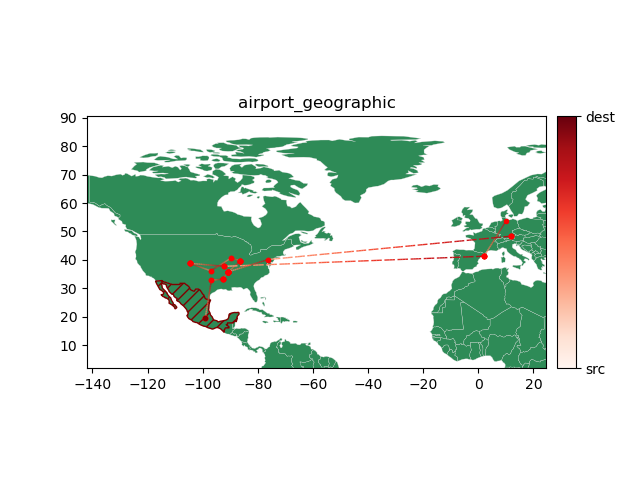
\includegraphics[width=0.8\linewidth]{DEU_0.png}
    \caption{DEU0}%
    \label{fig:DEU0}
\end{figure}


\bibliographystyle{unsrt}  
\bibliography{references}  

\end{document}

